%----------------------------------------------------------------------------------------
%	PACKAGES AND OTHER DOCUMENT CONFIGURATIONS
%----------------------------------------------------------------------------------------

\documentclass{article}

\usepackage{fancyhdr} % Required for custom headers
\usepackage{lastpage} % Required to determine the last page for the footer
\usepackage{extramarks} % Required for headers and footers
\usepackage{graphicx} % Required to insert images
\usepackage{amsmath, amssymb} % Required for Maths
\usepackage{mathtools} % Required for Maths
\usepackage{enumerate}
\usepackage{mathtools}
\usepackage{textcomp}
\usepackage{gensymb}
\usepackage{siunitx}
\usepackage{empheq}
\usepackage{ulem}
\usepackage{amssymb}

% Margins
\topmargin=-0.45in
\evensidemargin=0in
\oddsidemargin=0in
\textwidth=6.5in
\textheight=9.0in
\headsep=0.25in 

\linespread{1.1} % Line spacing

% Set up the header and footer
\pagestyle{fancy}
\lhead{\hmwkAuthorName} % Top left header
\chead{\hmwkClass\ (\hmwkClassInstructor\ \hmwkClassTime): \hmwkTitle} % Top center header
\rhead{\firstxmark} % Top right header
\lfoot{\lastxmark} % Bottom left footer
\cfoot{} % Bottom center footer
\rfoot{Page\ \thepage\ of\ \pageref{LastPage}} % Bottom right footer
\renewcommand\headrulewidth{0.4pt} % Size of the header rule
\renewcommand\footrulewidth{0.4pt} % Size of the footer rule

\setlength\parindent{0pt} % Removes all indentation from paragraphs

%----------------------------------------------------------------------------------------
%	DOCUMENT STRUCTURE COMMANDS
%	Skip this unless you know what you're doing
%----------------------------------------------------------------------------------------

% Header and footer for when a page split occurs within a problem environment
\newcommand{\enterProblemHeader}[1]{
\nobreak\extramarks{#1}{#1 continued on next page\ldots}\nobreak
\nobreak\extramarks{#1 (continued)}{#1 continued on next page\ldots}\nobreak
}

% Header and footer for when a page split occurs between problem environments
\newcommand{\exitProblemHeader}[1]{
\nobreak\extramarks{#1 (continued)}{#1 continued on next page\ldots}\nobreak
\nobreak\extramarks{#1}{}\nobreak
}

\setcounter{secnumdepth}{0} % Removes default section numbers
\newcounter{homeworkProblemCounter} % Creates a counter to keep track of the number of problems

\newcommand{\homeworkProblemName}{}
\newenvironment{homeworkProblem}[1][Problem \arabic{homeworkProblemCounter}]{ % Makes a new environment called homeworkProblem which takes 1 argument (custom name) but the default is "Problem #"
\stepcounter{homeworkProblemCounter} % Increase counter for number of problems
\renewcommand{\homeworkProblemName}{#1} % Assign \homeworkProblemName the name of the problem
\section{\homeworkProblemName} % Make a section in the document with the custom problem count
\enterProblemHeader{\homeworkProblemName} % Header and footer within the environment
}{
\exitProblemHeader{\homeworkProblemName} % Header and footer after the environment
}

\newcommand{\problemAnswer}[1]{ % Defines the problem answer command with the content as the only argument
\noindent\framebox[\columnwidth][c]{\begin{minipage}{0.98\columnwidth}#1\end{minipage}} % Makes the box around the problem answer and puts the content inside
}

\newcommand{\homeworkSectionName}{}
\newenvironment{homeworkSection}[1]{ % New environment for sections within homework problems, takes 1 argument - the name of the section
\renewcommand{\homeworkSectionName}{#1} % Assign \homeworkSectionName to the name of the section from the environment argument
\subsection{\homeworkSectionName} % Make a subsection with the custom name of the subsection
\enterProblemHeader{\homeworkProblemName\ [\homeworkSectionName]} % Header and footer within the environment
}{
\enterProblemHeader{\homeworkProblemName} % Header and footer after the environment
}

%----------------------------------------------------------------------------------------
%	NAME AND CLASS SECTION
%----------------------------------------------------------------------------------------

\newcommand{\hmwkTitle}{Homework\ \#3} % Assignment title
\newcommand{\hmwkDueDate}{Wednesday,\ October\ 14,\ 2015} % Due date
\newcommand{\hmwkClass}{ENPM 808M} % Course/class
\newcommand{\hmwkClassTime}{4:00 PM} % Class/lecture time
\newcommand{\hmwkClassInstructor}{Dr. William Levine} % Teacher/lecturer
\newcommand{\hmwkAuthorName}{Kanishka Ganguly} % Your name

%----------------------------------------------------------------------------------------
%	TITLE PAGE
%----------------------------------------------------------------------------------------

\title{
\vspace{2in}
\textmd{\textbf{\hmwkClass:\ \hmwkTitle}}\\
\normalsize\vspace{0.1in}\small{Due\ on\ \hmwkDueDate}\\
\vspace{0.1in}\large{\textit{\hmwkClassInstructor\ \hmwkClassTime}}
\vspace{3in}
}

\author{\textbf{\hmwkAuthorName}}
\date{} % Insert date here if you want it to appear below your name

%----------------------------------------------------------------------------------------

\begin{document}

\maketitle

%----------------------------------------------------------------------------------------
%	TABLE OF CONTENTS
%----------------------------------------------------------------------------------------

%\setcounter{tocdepth}{1} % Uncomment this line if you don't want subsections listed in the ToC

\newpage
\tableofcontents
\newpage

%----------------------------------------------------------------------------------------
%	PROBLEM 1
%----------------------------------------------------------------------------------------
\begin{homeworkProblem}
By definition, skew matrices have the following property:
\begin{align}
S + S^T = 0
\end{align}
We have
\begin{align}
e^A = I + A + \frac{1}{2} A^2 + \frac{1}{3!} A^3 + \dots\\
\implies e^S = I + S + \frac{1}{2} S^2 + \frac{1}{3!} S^3 + \dots\\
\implies {(e^S)}^T = {\big( I + S + \frac{1}{2} S^2 + \frac{1}{3!} S^3 + \dots \big)}^T\\
\implies {(e^S)}^T = e^{S^T}
\end{align}
Now, given $S \in so(3)$, we get from above
\begin{align}
(e^S)^T = {e^S}^T
\end{align}
Thus, we have
\begin{align}
e^S \times {e^S}^T = e^{S + S^T} = e^0 = I
\end{align}

Now, let $e^S = R$ which gives us
\begin{align}
RR^T = I
\end{align}
which is possible only when sum of the squares of each row $=1$, which is a property of $R \in SO(3)$.\\
This however gives us two possible determinant values for $R$, namely $+1$ or $-1$.\\

We also have 
\begin{align}
det(e^S) = e^{Tr(S)} = e^0 = 1
\end{align}
Thus, both conditions for $R \in SO(3)$ are met, namely
\begin{enumerate}
\item $RR^T = 1$
\item $det(R) = 1$
\end{enumerate}

Thus, $R = e^S \in SO(3)$.
\end{homeworkProblem}

%----------------------------------------------------------------------------------------
%	PROBLEM 2
%----------------------------------------------------------------------------------------

\begin{homeworkProblem} 
\problemAnswer{ % Answer
\begin{center}
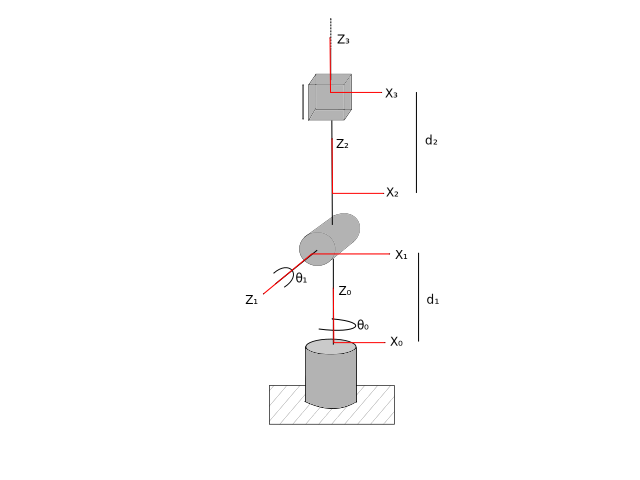
\includegraphics[width=0.75\columnwidth]{img/4-18.png} % Q2_1st Image
\end{center}
}
\vspace{20pt}
Choice of Axes - DH Convention

From given figure, we form DH Parameters as:
\begin{center}
\begin{tabular}{|l|l|l|l|l|{c}r}
\hline
Link ($i$) & $a_i$ & $\alpha_i$ & $d_i$ & $\theta_i$\\
\hline
1 & $0$ & $90$ & $d_1$ & $\mathbf{\theta_1}$\\
2 & $0$ & $90$ & $0$ & $\mathbf{\theta_2}$\\
3 & $0$ & $0$ & $\mathbf{d_2}$ & $0$\\
\hline
\end{tabular}
\end{center}
where \textbf{bold} indicates a variable parameter value.\\

We now have the following transformation matrices:
\begin{align}
T_1 =
\begin{bmatrix}
c_1 & 0 & s_1 & 0\\
s_1 & 0 & -c_1 & 0\\
0 & 1 & 0 & d_1\\
0 & 0 & 0 & 1
\end{bmatrix}\\
T_2 =
\begin{bmatrix}
c_2 & 0 & -s_2 & 0\\
s_2 & 0 & c_2 & 0\\
0 & -1 & 0 & 0\\
0 & 0 & 0 & 1
\end{bmatrix}\\
T_3 =
\begin{bmatrix}
1 & 0 & 0 & 0\\
0 & 1 & 0 & 0\\
0 & 0 & 1 & d_2\\
0 & 0 & 0 & 1
\end{bmatrix}
\end{align}

Taking products, we get:
\begin{align}
T_1 T_2=
\begin{bmatrix}
c_1 c_2 & -s_1 & -s_2 c_1 & 0\\
s_1 c_2 & c_1 & -s_2 s_1 & 0\\
s_2 & 0 & c_2 & d_1\\
0 & 0 & 0 & 1
\end{bmatrix}\\
T_1 T_2 T_3=
\begin{bmatrix}
c_1 c_2 & -s_1 & -s_2 c_1 & -s_2 c_1 d_2\\
s_1 c_2 & c_1 & -s_2 s_1 & -s_2 s_1 d_2\\
s_2 & 0 & c_2 & c_2 d_2 + d_1\\
0 & 0 & 0 & 1
\end{bmatrix}
\end{align}

From above matrices, we get:
\begin{align}
O_0 = {[0 \quad 0 \quad 0]}^T\\
O_1 = {[0 \quad 0 \quad d_1]}^T\\
O_2 = {[0 \quad 0 \quad d_1]}^T\\
O_3 = {[-s_2 c_1 d_2 \quad -s_2 s_1 d_2 \quad c_2 d_2 + d_1]}^T
\end{align}

Also, we have:
\begin{align}
Z_0 = 
\begin{bmatrix}
0 & 0 & 1
\end{bmatrix}^T\\
Z_1 = 
\begin{bmatrix}
s_1 & -c_1 & 0
\end{bmatrix}^T\\
Z_2 = 
\begin{bmatrix}
-s_2 c_1 & -s_2 s_1 & c_2
\end{bmatrix}^T\\
Z_3 = 
\begin{bmatrix}
-s_2 c_1 & -s_2 s_1 & c_2
\end{bmatrix}^T
\end{align}
From the figure, we have revolute joints at joints $1$ and $2$ and joint $3$ as prismatic joint. This gives us:
\begin{align}
J_1 =
\begin{bmatrix}
Z_0 \times (O_3 - O_0)\\
Z_0
\end{bmatrix}\\
J_2 =
\begin{bmatrix}
Z_1 \times (O_3 - O_1)\\
Z_1
\end{bmatrix}\\
J_3 =
\begin{bmatrix}
Z_2\\
0
\end{bmatrix}\\
J = [J_1 \quad J_2 \quad J_3]
\end{align}

We need to calculate $J_{11}$, which is the upper half of the matrix $J$. Thus,
\begin{align}
J_{11} = 
\begin{bmatrix}
\uline{Z_0 \times (O_3 - O_0)} & \uuline{Z_1 \times (O_3 - O_1)} & Z_2
\end{bmatrix}
\end{align}

For $\uline{Z_0 \times (O_3 - O_0)}$, we have
\begin{align}
(O_3 - O_0) = 
\begin{bmatrix}
-s_2 c_1 d_2\\
-s_2 s_1 d_2\\
c_2 d_2 + d_1
\end{bmatrix}\\
Z_0 \times (O_3 - O_0) = S(Z_0)(O_3 - O_0)\\
= 
\begin{bmatrix}
0 & -1 & 0\\
1 & 0 & 0 \\
0 & 0 & 0
\end{bmatrix}\times
\begin{bmatrix}
-s_2 c_1 d_2\\
-s_2 s_1 d_2\\
c_2 d_2 + d_1
\end{bmatrix}\\
\implies 
\begin{bmatrix}
s_2 s_1 d_2\\
-s2 c_1 d_2\\
0
\end{bmatrix}
\end{align}

For $\uuline{Z_1 \times (O_3 - O_1)}$, we have
\begin{align}
(O_3 - O_1) = 
\begin{bmatrix}
-s_2 c_1 d_2\\
-s_2 s_1 d_2\\
c_2 d_2
\end{bmatrix}\\
Z_1 \times (O_3 - O_1) = S(Z_1)(O_3 - O_1)\\
=
\begin{bmatrix}
0 & 0 & -c_1\\
0 & 0 & -s_1 \\
c_1 & s_1 & 0
\end{bmatrix}\times
\begin{bmatrix}
-s_2 c_1 d_2\\
-s_2 s_1 d_2\\
c_2 d_2
\end{bmatrix}\\
\implies 
\begin{bmatrix}
-c_1 c_2 d_2\\
-s1 c_2 d_2\\
-s_2 d_2
\end{bmatrix}
\end{align}

Combining results above, we get
\begin{align}
J_{11} = 
\begin{bmatrix}
s_2 s_1 d_2 & -c_1 c_2 d_2 & -s_2 c_1\\
-s_2 c_1 d_2 & -s_1 c_2 d_2 & -s_2 s_1\\
0 & -s_2 d_2 & c_2
\end{bmatrix}
\end{align}
\clearpage
\end{homeworkProblem}

%----------------------------------------------------------------------------------------
%	PROBLEM 3
%----------------------------------------------------------------------------------------

\begin{homeworkProblem}
\problemAnswer{ % Answer
\begin{center}
\includegraphics[width=0.75\columnwidth]{img/4-21.png} % Q3_1st Image
\end{center}
}
\vspace{20pt}
Choice of Axes - DH Convention

From given figure, we form DH Parameters as:
\begin{center}
\begin{tabular}{|l|l|l|l|l|{c}r}
\hline
Link ($i$) & $a_i$ & $\alpha_i$ & $d_i$ & $\theta_i$\\
\hline
1 & $0$ & $-90$ & $\mathbf{d_1}$ & $0$\\
2 & $0$ & $-90$ & $\mathbf{d_2}$ & $90$\\
3 & $0$ & $0$ & $\mathbf{d_3}$ & $0$\\
\hline
\end{tabular}
\end{center}
where \textbf{bold} indicates a variable parameter value.\\
We now have the following transformation matrices:
\begin{align}
T_1 =
\begin{bmatrix}
1 & 0 & 0 & 0\\
0 & 0 & 1 & 0\\
0 & -1 & 0 & d_1\\
0 & 0 & 0 & 1
\end{bmatrix}\\
T_2 =
\begin{bmatrix}
0 & 0 & -1 & 0\\
1 & 0 & 0 & 0\\
0 & -1 & 0 & d_2\\
0 & 0 & 0 & 1
\end{bmatrix}\\
T_3 =
\begin{bmatrix}
1 & 0 & 0 & 0\\
0 & 1 & 0 & 0\\
0 & 0 & 1 & d_3\\
0 & 0 & 0 & 1
\end{bmatrix}
\end{align}

Taking products, we get:
\begin{align}
T_1 T_2=
\begin{bmatrix}
0 & 0 & -1 & 0\\
0 & -1 & 0 & d_2\\
-1 & 0 & 0 & d_1\\
0 & 0 & 0 & 1
\end{bmatrix}\\
T_1 T_2 T_3=
\begin{bmatrix}
0 & 0 & -1 & d_3\\
0 & -1 & 0 & d_2\\
-1 & 0 & 0 & d_1\\
0 & 0 & 0 & 1
\end{bmatrix}
\end{align}

For a prismatic joint, we have
\begin{align}
J_i =
\begin{bmatrix}
Z_{i-1}\\
0
\end{bmatrix}\\
J = [J_1\quad J_2\quad J_3 \quad \dots]
\end{align}

We thus have:
\begin{align}
Z_0 = 
\begin{bmatrix}
0 & 0 & 1
\end{bmatrix}^T\\
Z_1 = 
\begin{bmatrix}
0 & 1 & 0
\end{bmatrix}^T\\
Z_2 = 
\begin{bmatrix}
-1 & 0 & 0
\end{bmatrix}^T\\
\therefore J = 
\begin{bmatrix}
Z_0 & Z_1 & Z_2\\
0 & 0 & 0
\end{bmatrix}\\
=
\begin{bmatrix}
0 & 0 & -1\\
0 & 1 & 0\\
1 & 0 & 0\\
0 & 0 & 0\\
0 & 0 & 0\\
0 & 0 & 0
\end{bmatrix}
\end{align}
We can see that $J$ is a $6 \times 3$ matrix. So, the maximum rank possible is $3$.\\
Since, the actual rank of $J$ is the maximum possible rank, we can say that \uuline{there are no singular configurations.}
\end{homeworkProblem}
\clearpage

%----------------------------------------------------------------------------------------
%	PROBLEM 4
%----------------------------------------------------------------------------------------

\begin{homeworkProblem}
From Equation 4.87 in the textbook, we have the following:
\begin{align}
B(\alpha) = 
\begin{bmatrix}
c_\phi s_\theta & -s_\phi & 0\\
s_\phi s_\theta & c_\phi & 0\\
c_\theta & 0 & 1
\end{bmatrix}
\end{align}
Taking the determinant of $B(\alpha)$ we get
\begin{align}
det(B(\alpha)) = (c_\phi s_\theta)(c_\phi)(1) + (-s_\phi)(0)(c_\theta) + (0)(s_\phi s_\theta)(0) - (0)(c_\phi)(c_\theta) - (-s_\phi)(s_\phi s_\theta)(1) - (c_\phi s_\theta)(0)(0)\\ 
\implies det(B(\alpha)) = (c_\phi s_\theta)(c_\phi) - (-s_\phi)(s_\phi s_\theta)\\
\implies det(B(\alpha)) = c^2_\phi s_\theta + s^2_\phi s_\theta\\
\implies det(B(\alpha)) = s_\theta
\end{align}
Now, given that $s_\theta \neq 0$, $det(B(\alpha)) = k$ where $k$ is some non-zero value.\\
\uuline{Thus $B(\alpha)$ is invertible if $s_\theta \neq 0$}
\end{homeworkProblem}
\clearpage
 \end{document}